\crefalias{section}{appendix}
\crefalias{subsection}{appendix}
\crefalias{subsubsection}{appendix}

\section{Schematic Overviews of Data Construction and Alignment }
\subsection{Data Construction Pipeline}
\label{app:data-construction-pipeline}
\Cref{fig:data-construction} illustrates the systematic pipeline for constructing the intervention-driven preference dataset. The process begins with initial event-time labeling using Gemini, which are then rigorously cross-verified: visual timestamps are validated through a consensus of GPT and Claude via frame-unit analysis, while acoustic timestamps undergo human inspection to ensure ground-truth reliability. 
After filtering samples based on strict agreement criteria, we apply three interventions, \shift, \mute, and \swap, to the validated source videos. This results in the final preference pairs, where the "chosen" response reflects true audio-visual grounding and the "rejected" response exposes the visually-plausible shortcuts we aim to mitigate during alignment.


\subsection{Intervention Summary}
\label{app:intervention_summary}
\Cref{tab:intervention-summary} summarizes the three interventions in \Thud. 
Each intervention keeps the visual stream fixed while perturbing the audio track to target one grounding dimension: \shift probes temporal synchronization, \mute probes sound existence, and \swap probes source consistency. 
These controlled cases test whether models verify the observed audio or simply infer plausible sounds from visual priors.

\begin{figure}[t]
    \centering
    \includegraphics[width=\linewidth]{Fig/DataDPO_splitAv3.pdf}
    \caption{
Pipeline for intervention \textcolor{pipelineblue}{\textbf{data construction}}. We create \shift, \mute, and \swap variants from source videos with salient acoustic events, annotate visual/audio events and timestamps via cross-model verification with human review, and construct chosen--rejected preference pairs for training. The bottom panel shows a representative \shift example.
}
    \label{fig:data-construction}
    \vspace{-0.3cm}
\end{figure}

\subsection{Preference Data Sources}
\label{app:recipe-data}

This section describes the preference data sources used in our alignment recipe study. Each preference example is represented as a pair of responses, where the chosen response provides the desired behavior and the rejected response provides a shortcut-prone or incorrect alternative.

\paragraph{Original synchronization preferences (OP).}
Original synchronization preferences are constructed from the annotated audio-visual event tuples introduced in \Cref{sec:AAPC}. For each video, we represent the aligned visual and acoustic event as
\begin{equation}
    z_i = (e_i^v, t_i^v, e_i^a, t_i^a),
\end{equation}
where $e_i^v$ and $t_i^v$ denote the visual event and its timestamp, while $e_i^a$ and $t_i^a$ denote the corresponding acoustic event and timestamp. The chosen response is the annotated answer derived from the original aligned event. The rejected response is produced by perturbing one or more components of $z_i$, such as the visual event, visual timestamp, acoustic event, or acoustic timestamp, creating a plausible but incorrect synchronization explanation.

\paragraph{SFT-policy negatives (SP).}
Self-sampled negatives are generated from the SFT model itself. Given the same video-question input, we use the reference annotation as the chosen response and treat the SFT model's incorrect or shortcut-prone output as the rejected response. This data source encourages the model to correct its own post-SFT failure modes.

\paragraph{Counterfactual temporal preferences (CTP).}
Counterfactual temporal preferences are constructed by pairing original and shifted videos. For an original video, the chosen response corresponds to the original synchronized condition, while the response describing the shifted condition is used as the rejected response. For a shifted video, this assignment is reversed: the shifted-condition answer is chosen, and the original synchronized answer is rejected. This forces the model to distinguish true temporal alignment from visually plausible but temporally inconsistent audio.

\paragraph{FineVideo descriptive preferences (FV-D).}
FV-D is derived from the FineVideo data described in \Cref{app:finevideo-data}. We use the description, localization, and attribution tasks, which encourage the model to produce faithful video descriptions, localize relevant events, and attribute answers to appropriate visual or audio evidence.

\paragraph{FineVideo audio-visual QA preferences (FV-AVQA).}
FV-AVQA corresponds to the audio-dependent QA subset in \Cref{app:finevideo-data}. These examples ask questions that require audio evidence. Candidate questions and answers are generated by Gemini and then manually filtered. We further retain examples where GPT-based text-only answering fails, since GPT does not receive the audio stream. This filtering emphasizes cases where the answer cannot be reliably inferred from visual or textual priors alone.

\paragraph{FineVideo audio-visual QA long-form preferences (FV-AVQA-L).}
FV-AVQA-L is a long-form version of FV-AVQA. Instead of only selecting an answer option, the chosen response includes both the answer and an explanation grounded in the audio-visual evidence. This data source encourages the model to justify audio-dependent answers rather than relying on short-form guesses.

\paragraph{LLaVA-Video multiple-choice QA (LV-MCQA).}
LV-MCQA is a multiple-choice video QA dataset titled LLaVA-Video-178K ~\cite{zhang2024videoinstructiontuningsynthetic}. We include it as a general video preference source to regularize the model toward broad video understanding and reduce over-specialization to intervention-style examples.


\subsection{Alignment Pipeline}
\label{app:alignment-pipeline}
\Cref{fig:preference_optimization} illustrates our two-stage post-training pipeline designed to detect \shift, \mute, and \swap failures while preserving general video understanding. 
The training process integrates our targeted intervention dataset and re-annotated general video instructions derived from FineVideo~\cite{Farre2024FineVideo}. 
In Stage 1, an SFT warm-up on intervention data establishes basic audio-aware patterns. Stage 2 applies DPO using a mixture of intervention preference pairs and general video data. The preference pairs teach the model to reject visually plausible shortcuts, while the general data acts as a regularizer to preserve broad multimodal capabilities.
\begin{figure}[t]
    \centering
    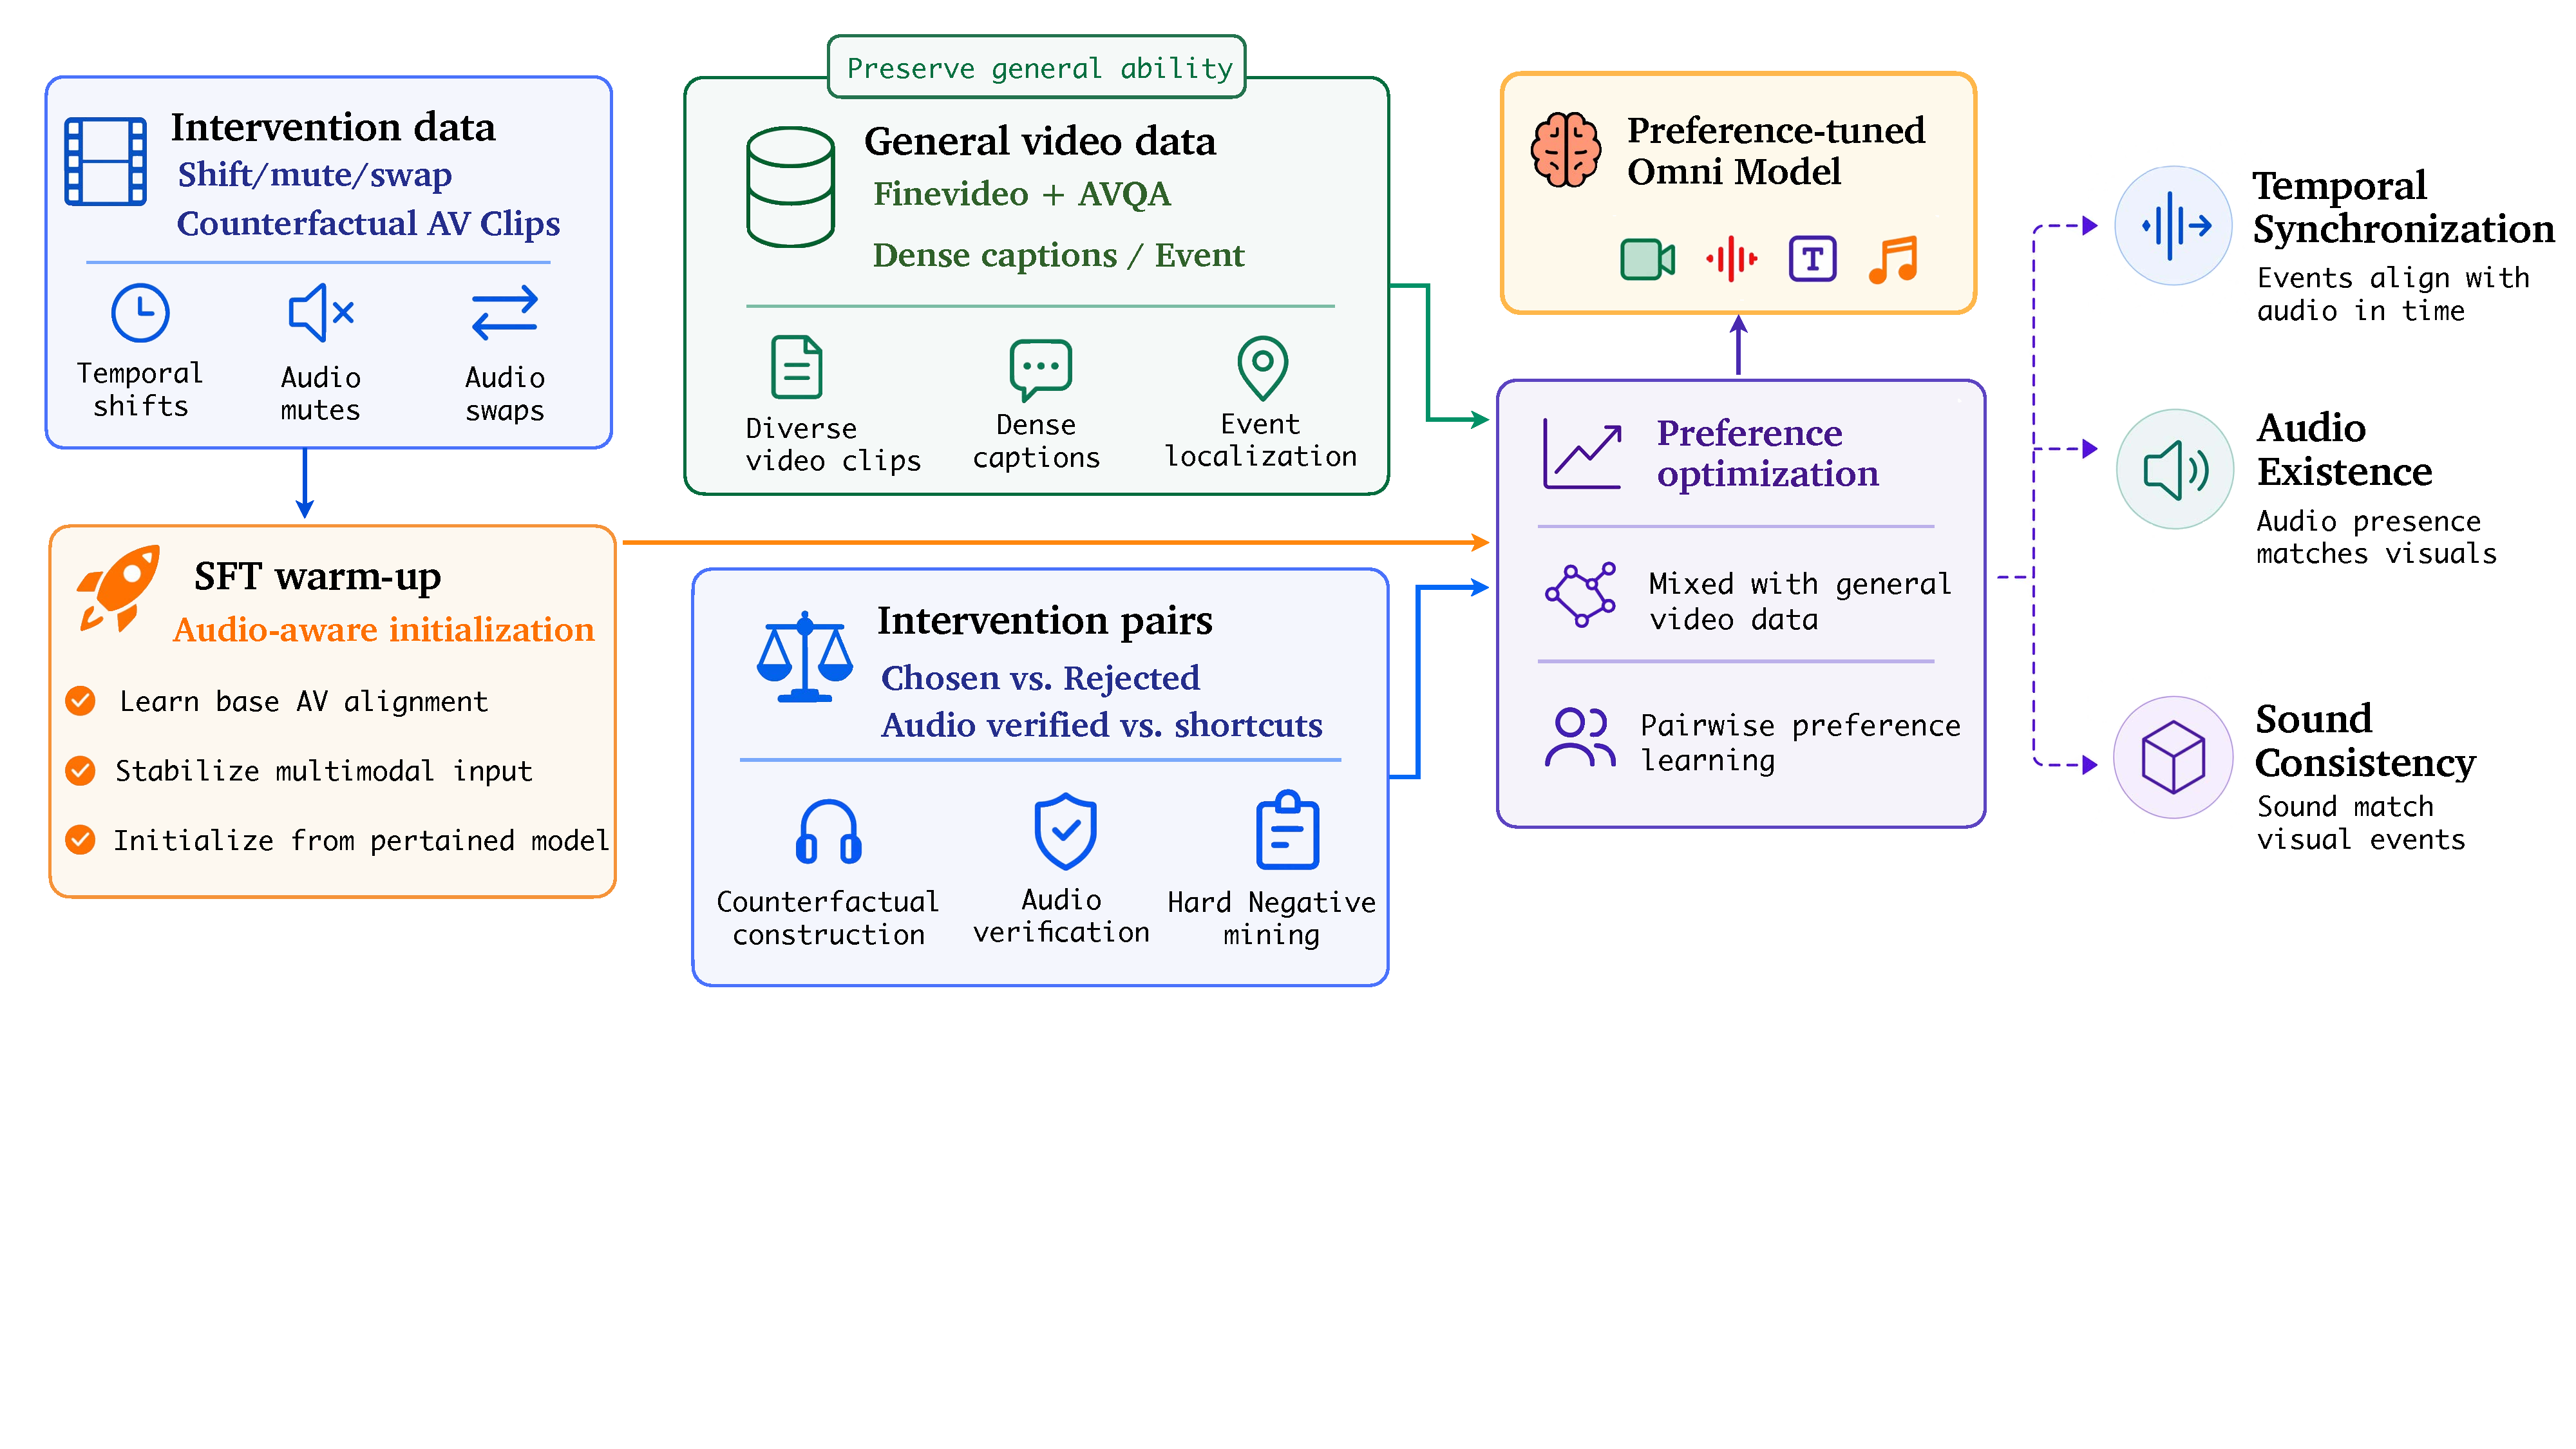
\includegraphics[width=\linewidth]{Fig/DataDPO_splitB_reduced.pdf}
   \caption{
Two-stage intervention-driven \textcolor{alignorange}{\textbf{alignment pipeline}}.
Counterfactual intervention data is first used for SFT warm-up, and intervention preference pairs are then mixed with general video data during preference optimization.
This design encourages audio-verified responses while preserving general video understanding.
}
    \label{fig:preference_optimization}
    \vspace{-1.0em}
\end{figure}


\begin{table}[h]
\caption{
Summary of our three physical interventions. Each intervention breaks a different natural audio-visual correlation and poses a diagnostic question about audio-visual grounding.
}
\label{tab:intervention-summary}
\centering
\begin{tabular}{lccc}
\toprule
\textbf{Intervention} 
& \textbf{Operation} 
& \textbf{Broken correlation}
& \textbf{Diagnostic question} \\
\midrule
\shift
& $a_{1:T} \rightarrow a_{1:T}^{+\Delta}$ 
& temporal synchrony
& Is the sound synchronized? \\
\mute 
& $a_{1:T} \rightarrow \varnothing$ 
& sound existence
& Is any sound present? \\
\swap
& $a_{1:T} \rightarrow a'_{1:T}$ 
& source consistency
& Does the sound match the event? \\
\bottomrule
\end{tabular}
\vspace{-0.5em}
\end{table}




%============================================
\section{Annotation and Verification Details}
\label{app:annotation}

\paragraph{Video-to-frame-unit conversion.}
For visual verification with GPT and Claude, we convert each video into $N$ temporally ordered frame units. Given a video of duration $T$ seconds, we split it into non-overlapping windows
\[
    u_j = [s_j, e_j], \qquad j=1,\ldots,N,
\]
where $s_j$ and $e_j$ denote the start and end time of the $j$-th unit. From each unit, we sample representative frames and present them in temporal order, together with the timestamp range of the unit. The verifier is asked to select the unit that contains the target visual event and optionally refine the timestamp within that unit. This frame-unit format allows models without direct video ingestion to perform temporal localization over visual evidence.

\paragraph{Gemini annotation prompt.}
We use Gemini to produce the initial audio-visual event annotation. The prompt is designed to avoid generic captioning and instead force event-level localization:
\begin{tcolorbox}[colback=gray!3,colframe=gray!35,boxrule=0.5pt,arc=2pt]
\small
You are given a video with audio. Identify the most salient visible event that has a corresponding acoustic consequence.  
Return a JSON object with the following fields:

\texttt{visual\_event}: a short description of the visible event.  

\texttt{visual\_time}: the timestamp in seconds when the visible event occurs.  

\texttt{audio\_event}: a short description of the corresponding sound.  

\texttt{audio\_time}: the timestamp in seconds when the sound occurs.  

\texttt{confidence}: high / medium / low.

If the visual event or audio event cannot be localized reliably, return \texttt{uncertain}.
\end{tcolorbox}

\paragraph{Frame-unit visual verification prompt.}
For GPT and Claude, we provide the ordered frame units and the candidate visual event proposed by Gemini:
\begin{tcolorbox}[colback=gray!3,colframe=gray!35,boxrule=0.5pt,arc=2pt]
\small
You are given temporally ordered frame units from a video. Each unit contains representative frames and a timestamp range.  
Target visual event: \texttt{[visual\_event]}.

Select the frame unit where this event occurs. 

Return:
\texttt{unit\_id}, \texttt{timestamp\_range}, and a one-sentence justification.  
If the event is not visible or cannot be localized, return \texttt{uncertain}.
\end{tcolorbox}

\paragraph{Agreement and filtering rules.}
We retain a sample only if it satisfies the following conditions:
\begin{enumerate}[leftmargin=1.5em,itemsep=2pt,topsep=2pt]
    \item \textbf{Visual agreement:} Gemini, GPT, and Claude localize the visual event within $\epsilon_v = 0.8$ seconds, or select overlapping frame units.
    \item \textbf{Audio verification:} the acoustic event is audible and its timestamp can be verified by human inspection within $\epsilon_a = 0.5$ seconds of the Gemini prediction.
    \item \textbf{Event clarity:} the visual event has a clear onset or peak moment, such as impact, fall, collision, breakage, or contact.
    \item \textbf{Acoustic salience:} the corresponding sound is not dominated by unrelated background music, speech, or noise.
    \item \textbf{Intervention validity:} after applying \shift, \mute, or \swap, the correct answer remains unambiguous.
\end{enumerate}

\paragraph{Manual review protocol.}
Samples failing automatic agreement are manually reviewed. We use the following decision rules. If the disagreement is due to a small boundary ambiguity, we correct the timestamp to the clearest event onset. If the visual event is partially occluded, spread over a long interval, or lacks a well-defined moment, we discard the sample. If the sound is too weak, masked by background noise, or not clearly tied to the visual event, we discard the sample. For \swap, we additionally discard cases where the substituted audio is trivially unrelated or too similar to the original audio; retained swaps must be acoustically plausible but inconsistent with the visible event.



% =============================================

\section{Experimental Configuration}
\label{app:experimental-configuration}

This section provides additional implementation details for our supervised fine-tuning (SFT), preference optimization, and evaluation experiments. All training experiments are conducted on 8*NVIDIA H200 GPUs, while evaluation experiments are conducted on either 8*NVIDIA H200 or 8*NVIDIA H100 GPUs. A single SFT run takes approximately 6 hours, and DPO training on 10K examples takes approximately 20 hours. For evaluation, the average inference time across the six datasets is approximately 5 hours per dataset.

\paragraph{Base model.}
We use Qwen3-Omni-30B-A3B-Instruct as the base omni-modal model. Video inputs are processed with audio enabled by setting \texttt{use\_audio\_in\_video=true}.

\paragraph{Training configuration.}
We summarize the training configurations for supervised fine-tuning and preference optimization in \Cref{tab:training-config}. Both stages are launched with \texttt{torchrun} on a single node with 8 GPUs, using DeepSpeed ZeRO-3 for memory-efficient distributed training. 

\begin{table}[t]
\centering
\caption{Training configurations for the supervised fine-tuning and DPO stages.}
\vspace{3pt}
\label{tab:training-config}
\footnotesize
\setlength{\tabcolsep}{5pt}
\renewcommand{\arraystretch}{1.12}
\begin{tabular}{p{0.24\linewidth}p{0.34\linewidth}p{0.34\linewidth}}
\toprule
\textbf{Configuration} & \textbf{SFT} & \textbf{DPO} \\
\midrule
Initialization 
& Qwen3-Omni-30B-A3B-Instruct 
& SFT checkpoint \\
Fine-tuning type 
& Full-parameter tuning 
& LoRA \\
Epochs 
& 3 
& 1 \\
\midrule
Learning rate 
& $2\times 10^{-6}$ 
& $1\times 10^{-6}$ \\
Scheduler / warmup 
& Cosine / 0.03 
& Cosine / 0.03 \\
Weight decay / grad norm 
& 0.01 / 1.0 
& 0.0 / 1.0 \\
Precision 
& bf16 
& bf16 \\
\midrule
Cutoff length 
& 131,072 
& 131,072 \\
Video max pixels 
& 501,760 
& 250,880 \\
Audio in video 
& Enabled 
& Enabled \\
\midrule
Batch size 
& 1 per GPU; accum. 4; effective 32 
& 1 per GPU; accum. 8; effective 64 \\
Memory optimization 
& DeepSpeed ZeRO-3 
& DeepSpeed ZeRO-3 \\
\midrule
Preference loss 
& -- 
& Sigmoid DPO, $\beta=0.1$ \\
LoRA setting 
& -- 
& rank 32; alpha 64; dropout 0.05 \\
\midrule
Workers 
& 16 preprocessing; 8 dataloader 
& 16 preprocessing; 8 dataloader \\
Distributed setup 
& 8 GPUs, single node 
& 8 GPUs, single node \\
Hardware 
& H200 GPUs 
& H200 GPUs \\
\bottomrule
\end{tabular}
\end{table}

% =============================================
\section{Preference Pair Examples}
\label{app:preference_examples}

\begin{tcolorbox}[
colback=gray!3,
colframe=gray!35,
title=\textbf{Examples of Preference Pair Construction},
fonttitle=\small,
coltitle=black,
boxrule=0.6pt,
arc=2pt,
left=5pt,
right=5pt,
top=5pt,
bottom=5pt
]
% \small
\begin{tabularx}{\linewidth}{p{0.10\linewidth} X}
\shift
&
\textbf{Chosen:} The visible fall occurs at $\sim 5.0$s, while the impact sound is heard at $\sim 3.1$s, indicating a synchronization mismatch. \\
&
\textbf{Rejected:} The sound is synchronized with the fall. \\

\specialrule{0.3pt}{4pt}{4pt}

\mute
&
\textbf{Chosen:} The audio track is silent throughout the clip; no music, speech, ambient noise, or sound effects are detected. \\
&
\textbf{Rejected:} The animated music-video scene is described as containing female vocals, a chaotic electronic rock beat, rain, thunder, TV static, and glass-shattering effects. \\

\specialrule{0.3pt}{4pt}{4pt}

\swap
&
\textbf{Chosen:} The visuals show an optics diffraction demonstration, but the audio describes how to use a centrifuge, indicating an audio-source mismatch. \\
&
\textbf{Rejected:} The narrator explains the diffraction setup as the hand shines a smartphone light through the pen tip. \\

\end{tabularx}
\end{tcolorbox}


\section{FineVideo-derived general instruction data}
\label{app:finevideo-data}

\begin{tcolorbox}[
colback=gray!2,
colframe=gray!35,
boxrule=0.6pt,
arc=2pt,
left=5pt,
right=5pt,
top=5pt,
bottom=5pt
]
\small
\vspace{4pt}

\noindent
\begin{minipage}[t]{0.49\linewidth}
\begin{tcolorbox}[
colback=descBlue,
colframe=descBlueLine,
boxrule=0.45pt,
arc=2pt,
left=5pt,
right=5pt,
top=4pt,
bottom=4pt
]
\textbf{Description}\\
Describe visible events and audible cues.
\end{tcolorbox}
\end{minipage}
\hfill
\begin{minipage}[t]{0.49\linewidth}
\begin{tcolorbox}[
colback=locGreen,
colframe=locGreenLine,
boxrule=0.45pt,
arc=2pt,
left=5pt,
right=5pt,
top=4pt,
bottom=4pt
]
\textbf{Localization}\\
Locate visual/audio events in time.
\end{tcolorbox}
\end{minipage}

\vspace{3pt}

\noindent
\begin{minipage}[t]{0.49\linewidth}
\begin{tcolorbox}[
colback=attrPurple,
colframe=attrPurpleLine,
boxrule=0.45pt,
arc=2pt,
left=5pt,
right=5pt,
top=4pt,
bottom=4pt
]
\textbf{Attribution}\\
Infer the source or material of a cue.
\end{tcolorbox}
\end{minipage}
\hfill
\begin{minipage}[t]{0.49\linewidth}
\begin{tcolorbox}[
colback=qaOrange,
colframe=qaOrangeLine,
boxrule=0.45pt,
arc=2pt,
left=5pt,
right=5pt,
top=4pt,
bottom=4pt
]
\textbf{Audio-dependent QA}\\
Answer questions that require audio evidence.
\end{tcolorbox}
\end{minipage}

\end{tcolorbox}






% ==== Appendix content ====
\section{Qualitative GPT-5.5 Outputs (Visual-Only Input)}
\label{app:gpt-qualitative}

We provide representative raw outputs of GPT-5.5 across the three tasks of our
test data---\mute, \shift, and \swap---when the model
is given visual frames only. Since the model does not have access to the
audio track, these examples illustrate how it tends to respond when forced to
reason about audio without being able to hear it.

% ---------------- Mute ----------------
\begin{tcolorbox}[gptbox,title={Task: \mute \textemdash{} What does the audio sound like?}]
\begin{tcolorbox}[videoline]
video: Bats \& Balls Fail Compilation 47.mp4
\end{tcolorbox}
\textbf{GPT-5.5 raw output:}\\
\textit{``The audio is likely from an indoor gym: basketball dribbles and
sneaker squeaks as someone runs toward the hoop, followed by the thud/clank
of a dunk attempt. Then there's a sudden loud crash as the backboard
shatters, with glass raining down onto the floor. You can hear startled
reactions---shouting, laughter, and movement---as people react and run over
afterward.''}
\end{tcolorbox}

% ---------------- Sync ----------------
\begin{tcolorbox}[gptbox,title={Task: \shift \textemdash{} Is the audio in sync with the video?}]
\begin{tcolorbox}[videoline]
video: Are You Serious! - Throwback Thursday Sept 2017 11\_delay\_2.39s.mp4
\end{tcolorbox}
\textbf{GPT-5.5 raw output:}\\
\textit{``The audio and video appear to be synchronized.\\[2pt]
The clearest sync points are the physical impact moments: the man's
jump/trip over the boards, the body hitting the ground, and the subsequent
movement/laughter reaction. The impact sound lines up with the visual fall
closely enough that I do not perceive a meaningful lead or lag. Any offset,
if present, seems very small---likely under about 0.1--0.2 seconds---and not
enough to call the tracks out of sync.''}
\end{tcolorbox}

% ---------------- Swap ----------------
\begin{tcolorbox}[gptbox,title={Task: \swap \textemdash{} Does the audio match the video content?}]
\begin{tcolorbox}[videoline]
video: Bats \& Balls Fail Compilation 47.mp4 \\
audio swapped from: FailArmy After Dark - That's Going To Cost You Ep.\,10 (103.mp4)
\end{tcolorbox}
\textbf{GPT-5.5 raw output:}\\
\textit{``yes''}
\end{tcolorbox}


\section{Evaluation Prompts}
\label{app:prompts}

This section documents the exact prompts used to elicit model responses on
each of the three tasks, together with the GPT-based judge prompts used to
parse those free-form responses into a structured prediction. For
\textsc{Mute} and \textsc{Swap}, the numbers reported in the main text
correspond to the \emph{neutral} prompt setting, in which the model is asked
an open-ended description question rather than being directly cued about the
hypothesis under test. For \textsc{Shift}, a single structured prompt is used,
which simultaneously asks the model to make an aligned/misaligned decision
and estimate the offset.

\subsection{Average Gap Calculation}
We summarize shortcut reliance by the average accuracy drop from each non-intervened control to its paired counterfactual condition:
\begin{equation}
\Delta_{\mathrm{shortcut}}
=
\frac{1}{|\mathcal{D}|}
\sum_{d \in \mathcal{D}}
\left(
\mathrm{Acc}_{\mathrm{Orig},d}
-
\mathrm{Acc}_{\mathrm{Interv},d}
\right),
\quad
\mathcal{D}=\{\mathrm{Sync}, \mathrm{Exist.}, \mathrm{Consist.}\}.
\end{equation}
Larger values indicate a larger performance collapse under counterfactual interventions. We report the gap only when all three dimensions are available. For free-form outputs, GPT-5.4 is used as an LLM judge to adjudicate predicted labels.

\subsection{Inference Prompts}

% ---- Mute ----
\begin{tcolorbox}[promptbox,title={\textsc{Mute} \textemdash{} Inference Prompt}]
\textit{``Describe the audio you hear in this video.''}
\end{tcolorbox}

% ---- Swap ----
\begin{tcolorbox}[promptbox,title={\textsc{Swap} \textemdash{} Inference Prompt}]
\textit{``Describe what you see in the video and what you hear in the audio.''}
\end{tcolorbox}

% ---- Shift ----
\begin{tcolorbox}[promptbox,title={\textsc{Shift} \textemdash{} Inference Prompt}]
\textit{``Watch this video and listen to its audio carefully. Determine
whether the audio and video tracks are synchronized. If they are not
synchronized, identify the direction of the offset (audio delayed or audio
early relative to video) and estimate the offset in seconds. Explain your
reasoning.''}
\end{tcolorbox}

\subsection{GPT Judge Prompts}

Because the inference prompts above elicit free-form text, we use GPT as a
structured-output extractor to convert each response into a discrete
prediction. The judge is prompted with the system message below and given the
model's raw response as the user message; it is required to return a single
JSON object.

% ---- Mute judge ----
\begin{tcolorbox}[judgebox,title={\textsc{Mute} \textemdash{} Judge System Prompt}]
\textit{``You are evaluating a model's response about a video whose audio has
been secretly replaced with silence. The user will give you the model's
response. Classify the model's assessment into exactly ONE of four categories
and return ONLY valid JSON (no markdown, no explanation):}\\[2pt]
\texttt{\{"prediction": "synced"|"delay"|"early"|"muted", "explanation":
"<one sentence>"\}}\\[2pt]
\textit{Rules:}
\begin{itemize}\itemsep0pt
  \item \textit{``synced'': the model claims audio and video are
        synchronized (it is hallucinating audio).}
  \item \textit{``delay'': the model claims audio is delayed relative to
        video (hallucinating audio + claiming offset).}
  \item \textit{``early'': the model claims audio is early relative to video
        (hallucinating audio + claiming offset).}
  \item \textit{``muted'': the model states there is no audio, the audio is
        silent, muted, or absent.}
  \item \textit{If the model describes specific sounds (e.g.\ ``thud'',
        ``music'', ``splash'') but does not explicitly say the video is
        silent, classify based on its sync/desync conclusion, not as
        ``muted''.}
  \item \textit{If the model is ambiguous or gives no clear answer, default
        to ``synced''.''}
\end{itemize}
\end{tcolorbox}

% ---- Swap judge ----
\begin{tcolorbox}[judgebox,title={\textsc{Swap} \textemdash{} Judge System Prompt}]
\textit{``You are evaluating a model's response about a video whose audio
has been secretly replaced with audio from a DIFFERENT unrelated video. The
user will give you the model's response. Classify the model's assessment
into exactly ONE of four categories and return ONLY valid JSON (no markdown,
no explanation):}\\[2pt]
\texttt{\{"prediction": "synced"|"delay"|"early"|"mismatched",
"explanation": "<one sentence>"\}}\\[2pt]
\textit{Rules:}
\begin{itemize}\itemsep0pt
  \item \textit{``mismatched'': the model says the audio does NOT match the
        visual content, or the audio and video are unrelated, or the sounds
        don't correspond to what's shown.}
  \item \textit{``synced'': the model claims audio and video are well
        synchronized and matching.}
  \item \textit{``delay'': the model claims audio is delayed (but still
        believes they match semantically).}
  \item \textit{``early'': the model claims audio is early (but still
        believes they match semantically).}
  \item \textit{Prefer ``mismatched'' whenever the model expresses
        confusion, doubt about the audio matching the video, or says the
        audio seems unrelated.}
  \item \textit{Default to ``synced'' if the answer is ambiguous.''}
\end{itemize}
\end{tcolorbox}

% ---- Shift judge ----
\begin{tcolorbox}[judgebox,title={\textsc{Shift} \textemdash{} Judge System Prompt}]
\textit{``You are a structured-output extractor. The user will give you a
model's free-text response about audio-video synchronization. Extract the
following fields and return ONLY valid JSON (no markdown, no explanation):}
\\[2pt]
\texttt{\{"synced": <bool>, "direction": "none"|"delay"|"early",
"offset\_sec": <float>, "t\_v": <float or null>, "t\_a": <float or null>,
"explanation": "<one sentence>"\}}\\[2pt]
\textit{Rules:}
\begin{itemize}\itemsep0pt
  \item \textit{synced: true if the model says audio and video are
        synchronized, false otherwise.}
  \item \textit{direction: ``delay'' means audio comes AFTER the visual
        event; ``early'' means audio comes BEFORE the visual event; ``none''
        if synced is true.}
  \item \textit{offset\_sec: estimated time gap in seconds. 0.0 if synced.}
  \item \textit{t\_v: the timestamp (in seconds) the model attributes to
        the VISUAL event. null if not mentioned.}
  \item \textit{t\_a: the timestamp (in seconds) the model attributes to
        the AUDIO event. null if not mentioned.}
  \item \textit{If you cannot determine a field, use the default (true /
        ``none'' / 0.0 / null / ``'').''}
\end{itemize}
\end{tcolorbox}



%================================
\section{Failure-mode definitions}
\label{app:failure-modes}

This appendix provides the detailed definition and measurement protocol for
each of the eight failure modes reported in
\Cref{fig:failure_heatmap}. All rates lie in $[0,1]$; higher values
indicate more frequent failures. Free-form (neutral-prompt) responses are
classified by an independent OpenAI GPT-5.4 judge so that the mute/swap modes
do not depend on a model self-reporting its own confusion.

\paragraph{A. Audio Hallucination.}
Errors in which the model invents or accepts audio content that is
incompatible with the input.

\begin{description}
  \item[Mute Hallucination.] On videos whose audio track has been replaced
    with silence, the prompt is \textit{``Describe the audio you hear in this
    video.''} The judge classifies each response into
    \texttt{muted} / \texttt{audio\_described} / \texttt{visual\_only}, and
    \emph{Mute Hallucination} is the \texttt{audio\_described} rate: the
    fraction of responses in which the model produces any concrete description
    of audio content (speech, music, ambient noise, impacts) instead of
    reporting silence.

  \item[Swap False-Match.] On videos whose audio track has been replaced with
    the soundtrack of an unrelated video, the prompt is \textit{``Describe
    what you see in the video and what you hear in the audio.''}
    \emph{Swap False-Match} is the fraction of responses in which the judge
    concludes the model treated the (mismatched) audio as a plausible natural
    match for the visuals.
\end{description}

\paragraph{B.\ Audio Denial.}
Symmetric errors on naturally paired (un-intervened) videos.

\begin{description}
  \item[False Silence.] On videos with their original audio, the same neutral
    mute prompt is used. \emph{False Silence} is the fraction of responses in
    which the model claims silence or ``no audible content'' despite real
    audio being present.

  \item[Swap False-Mismatch.] On videos with their original audio, the same
    neutral swap prompt is used. \emph{Swap False-Mismatch} is the fraction
    of responses in which the model spuriously claims an audio--visual
    mismatch on a naturally synchronized pair.
\end{description}

\paragraph{C.\ Question Avoidance.}

\begin{description}
  \item[Audio Dodge.] Fraction of responses to the neutral mute prompt in
    which the model produces a visual-only description and never engages with
    the audio question (neither describes any sound nor claims silence). We
    report the mean of this rate across the intervention (silenced) and
    control (real audio) conditions because non-engagement is a property of
    the model, not of whether audio is real.
\end{description}

\paragraph{D.\ Temporal Failures (sync task).}
The sync benchmark contains synced originals together with two intervention
variants per video: an audio-delayed copy (\textsc{delay}) and an
audio-advanced copy (\textsc{early}), both with offsets of approximately
$\pm 2$\,s. Each model's free-form response is parsed by the judge into a
boolean \texttt{pred\_synced} and a categorical
$\texttt{pred\_direction}\in\{\textsc{delay},\textsc{early},\textsc{none}\}$.

\begin{description}
  \item[Offset Blindness.] Fraction of desync samples (delay or early) for
    which the model judges the clip to be synced. This isolates pure failure
    to perceive temporal misalignment.

  \item[Direction Confusion.] Among the desync samples on which the model
    correctly judges the clip to be non-synced, the fraction for which it
    picks the \emph{wrong} direction (calls a delay an early or vice versa).
    This isolates direction-of-offset perception from offset detection
    itself.

  \item[False Sync Alarm.] Fraction of synced original samples for which the
    model claims the clip is desynced. Symmetric counterpart to Offset
    Blindness: false alarms on naturally aligned audio.
\end{description}

For Gemini-3.1-pro, per-row sync predictions were not retained, so its
Offset Blindness, Direction Confusion, and False Sync Alarm are derived from
the aggregate \texttt{sync\_desync\_accuracy},
\texttt{direction\_accuracy\_on\_desync}, and per-category accuracies in the
saved \texttt{metrics.json}, which are mathematically equivalent to the
per-row counts.





% ================================================
\section{Limitations.}
\label{app:limit}
Our training recipe is currently evaluated on a limited set of base models, so its effectiveness across broader omni-modal model families remains to be further studied. In addition, our recipe experiments primarily validate the effect of applying DPO after SFT for improving temporal synchronization. We have not yet conducted a complete training study for the Mute and Swap settings, which probe audio existence and cross-modal consistency. Extending the recipe to these intervention types is an important direction for future work.

\section{Ethics and Broader Impacts}
\label{app:ethics-impact}

\subsection{Ethics.}
Our research follows the NeurIPS Code of Ethics. The study is designed as a diagnostic and alignment analysis of audio-visual grounding in multimodal models, and does not involve human-subject experiments, crowdsourcing, or the collection of personally identifiable information. The video data used in our experiments comes from public or properly licensed sources, and we use the data only for model evaluation and training under controlled audio-visual interventions. Our analysis does not perform face recognition, identity inference, biometric classification, or any other person-level profiling.

\subsection{Broader Impacts}
\paragraph{Positive impacts.}
This work aims to improve the reliability of video-capable multimodal and omni-modal models by revealing when they rely on visual-semantic shortcuts rather than genuine audio-visual verification. By introducing controlled Mute, Swap, and Shift interventions, our evaluation can help researchers diagnose pseudo-alignment and develop models that more faithfully check whether audio is present, synchronized, and consistent with the visual scene. Such improvements may benefit downstream applications where audio-visual grounding is important, including assistive technologies, video understanding, human-computer interaction, and safety-critical multimodal monitoring.

\paragraph{Potential risks and mitigations.}
The main risk is that intervention-based diagnostics could be used to construct adversarial examples or to optimize models specifically for benchmark performance rather than robust real-world grounding. In addition, improved audio-visual verification does not eliminate all hallucination risks, and deployed systems may still fail under out-of-distribution sounds, noisy environments, edited videos, or subtle cross-modal inconsistencies. To mitigate these risks, we frame our benchmark as a diagnostic tool rather than a deployment guarantee, report limitations of the evaluated settings, and encourage evaluating models under diverse interventions instead of relying on aggregate accuracy alone. If releasing data or code, we will document intended use, licenses, and limitations, and avoid releasing sensitive or personally identifying content.

\section{New Assets}
\label{app:assets}

We introduce intervention-based evaluation assets for probing audio-visual grounding under three controlled settings: Mute, Swap, and Shift. These assets are intended for diagnostic evaluation, testing whether multimodal models verify the audio stream rather than relying on visual-semantic shortcuts.

For each selected video, we construct intervention variants by modifying only the audio stream. Mute removes the audio track to test audio-existence verification. Swap replaces the original audio with mismatched audio to test cross-modal consistency. Shift temporally displaces the audio to test synchronization and offset reasoning. Each example is paired with its intervention type, evaluation condition, and target label.

The assets are verified by members of the research team to ensure that the intervention is valid and the label is unambiguous. We reject examples with unclear visual events, corrupted or inaudible audio, failed interventions, or ambiguous labels. The assets are used only for model evaluation and alignment research, and are not intended as a guarantee of real-world robustness. Their limitations include restricted intervention coverage, possible residual annotation noise, and limited coverage of all real-world audio-visual failure modes.